% RM =====================================================================================
\begin{frame}
	\section{Research Methodology}
	\setbeamercolor{block title example}{use=structure,fg=white,bg=blue!80!black}
	\begin{beamercolorbox}[rounded=true]{block title example}
		\centering
		\LARGE
		Research Methodology
	\end{beamercolorbox}
\end{frame}


\begin{frame}
	\frametitle{Research Methodology}
	The experiment consists of step below.
	\begin{itemize}
		\item<1-> Mobile Robot and Sensor Model
		\item<2-> Occupancy Grid Map
		\item<3-> Path Planning
		\item<4-> Control
	\end{itemize}
\end{frame}


\begin{frame}
	\subsection{Mobile Robot and Sensor Model}
	\setbeamercolor{block title example}{use=structure,fg=white,bg=blue!80!black}
	\begin{beamercolorbox}[rounded=true]{block title example}
		\centering
		\LARGE
		Mobile Robot and Sensor Model
	\end{beamercolorbox}
\end{frame}


\begin{frame}
	\frametitle{Mobile Robot and Sensor Model}
	\framesubtitle{Mobile Robot and Sensor Type}
	\begin{columns}
		\column{0.5\textwidth}
		\begin{figure}
			\caption{Differential Drive Robot\footnotemark}
			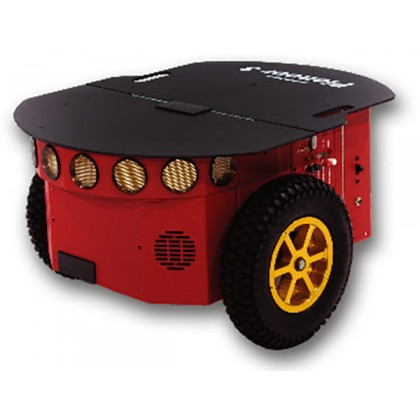
\includegraphics[scale=0.3]{image/DDWMR.jpg}
		\end{figure}
		
		\column{0.5\textwidth}
		Those sensors are:
		\begin{itemize}
			\item Wheel Encoder
			\item Light Detecting and Ranging Sensor (LIDAR)
			\item Inertial Measurement Unit (IMU)
		\end{itemize}
	\end{columns}
\footnotetext[4]{Pioneer P3-DX,https://www.generationrobots.com/en/402395-robot-mobile-pioneer-3-dx.html}
\end{frame}


\begin{frame}
	\frametitle{Mobile Robot and Sensor Model}
	\framesubtitle{Mobile Robot Kinematic Model}
	Kinematic model describes the robot velocities in the local frame to global frame.
	\begin{columns}
		\column{0.5\textwidth}
		\begin{figure}
			\caption{Differential Drive Kinematic Model}
			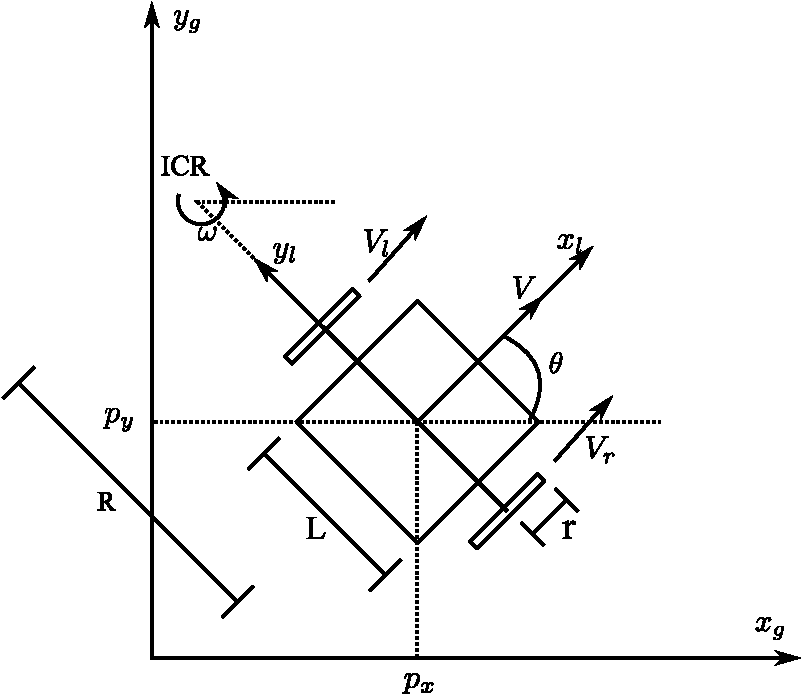
\includegraphics[scale=0.43]{image/DDWMR_kine.pdf}
		\end{figure}
		
		\column{0.5\textwidth}
		Where:
		\begin{itemize}
			\item {\makebox[1cm]{(\(x_g,y_g\))\hfill} is global frame}
			\item {\makebox[1cm]{(\(x_l,y_l\))\hfill} is local frame}
			\item {\makebox[1cm]{\(r\)\hfill} is wheel radius}
			\item {\makebox[1cm]{\(L\)\hfill} is robot base length}
			\item {\makebox[1cm]{\(V_l\&V_r\)\hfill} is left and right wheel linear velocity}
			\item {\makebox[1cm]{\(V\)\hfill} is linear velocity}
			\item {\makebox[1cm]{\(\omega\)\hfill} is angular velocity }
		\end{itemize}
	\end{columns}
\end{frame}


\begin{frame}
	\frametitle{Mobile Robot and Sensor Model}
	\framesubtitle{Sensor Model}
	\footnotesize
	\begin{columns}
		\column{0.7\textwidth}
	%Robot velocity in global frame is:
	\begin{block}{\footnotesize Robot global frame velocity in continueous time step}
		\begin{equation}
			\dot{x}(t)=
			\begin{bmatrix}
				\dot{p_x}(t) \\
				\dot{p_y}(t) \\
				\dot{\theta}(t)
			\end{bmatrix} = 
			\begin{bmatrix}
				cos(\theta(t)) && 0\\
				sin(\theta(t)) && 0\\
				0 && 1
			\end{bmatrix}
			\begin{bmatrix}
				V(t)\\
				\omega(t)
			\end{bmatrix}
		\end{equation}
	\end{block}

	\begin{block}{\footnotesize Robot Velocity}
		\begin{equation}
			\begin{bmatrix}
				V\\
				\omega
			\end{bmatrix}=\begin{bmatrix}
				\frac{r}{2} & \frac{r}{2}\\
				\frac{r}{L} & -\frac{r}{L}
			\end{bmatrix}\begin{bmatrix}
				\omega_r\\
				\omega_l
			\end{bmatrix}
		\end{equation}
	\end{block}

	\begin{block}{\footnotesize Predicted Robot Pose}
		\begin{equation}
			\hat{x}^-_k=
			\begin{bmatrix}
				p_{x,k}\\
				p_{y,k}\\
				\theta_k
			\end{bmatrix}=\begin{bmatrix}
				p_{x,k-1}\\
				p_{y,k-1}\\
				\theta_{k-1}
			\end{bmatrix}+\begin{bmatrix}
				cos(\theta_{k-1}) T_s && 0\\
				sin(\theta_{k-1}) T_s && 0\\
				0 && T_s
			\end{bmatrix}
			\begin{bmatrix}
				V_{k-1}\\
				\omega_{k-1}
			\end{bmatrix}
		\end{equation}
	\end{block}
	
	
	\column{0.2\textwidth}
	\textbf{Wheel Encoder} measures the rotation velocity of each wheel denoted by \(\omega_r\) and \(\omega_l\).
	\begin{figure}
		\caption{Encoder}
		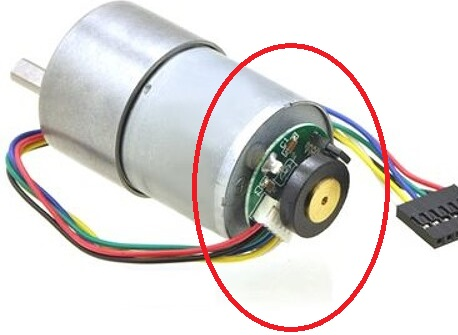
\includegraphics[scale=0.2]{image/encoder}
	\end{figure}
	\end{columns}
\end{frame}



%\begin{frame}
%	\frametitle{Mobile Robot and Sensor Model}
%	\framesubtitle{Sensor Model}
%	\textbf{Wheel Encoder} measures the rotation velocity of each wheel denoted by \(\omega_r\) and \(\omega_l\).
%	\begin{columns}
%		\column{0.5\textwidth}
%		\begin{block}{Robot Velocity}
%			\begin{equation}
%				\begin{bmatrix}
%					V\\
%					\omega
%				\end{bmatrix}=\begin{bmatrix}
%					\frac{r}{2} & \frac{r}{2}\\
%					\frac{r}{L} & -\frac{r}{L}
%				\end{bmatrix}\begin{bmatrix}
%					\omega_r\\
%					\omega_l
%				\end{bmatrix}
%			\end{equation}
%		\end{block}
%		\column{0.5\textwidth}
%		\begin{figure}
%			\caption{Encoder}
%			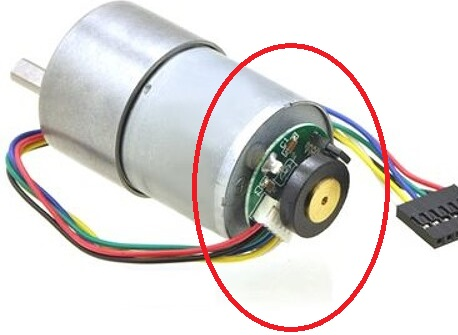
\includegraphics[scale=0.2]{image/encoder}
%		\end{figure}
%	\end{columns}
%	\begin{block}{Predicted Robot Pose}
%		\begin{equation}
%			\hat{x}^-_k=
%			\begin{bmatrix}
%				p_{x,k}\\
%				p_{y,k}\\
%				\theta_k
%			\end{bmatrix}=\begin{bmatrix}
%				p_{x,k-1}\\
%				p_{y,k-1}\\
%				\theta_{k-1}
%			\end{bmatrix}+\begin{bmatrix}
%				cos(\theta_{k-1}) T_s && 0\\
%				sin(\theta_{k-1}) T_s && 0\\
%				0 && T_s
%			\end{bmatrix}
%			\begin{bmatrix}
%				V_{k-1}\\
%				\omega_{k-1}
%			\end{bmatrix}
%		\end{equation}
%	\end{block}
%\end{frame}


\begin{frame}
	\frametitle{Mobile Robot and Sensor Model}
	\framesubtitle{Sensor Model}
	\textbf{LIDAR} data is input to LidarScanMatch that give the measurement of robot position \(p_x\) and \(p_y\).\\
	\hspace{\linewidth}\\
	\textbf{IMU} measures the robot orientation by integrate IMU gyroscope in z-axis \(\omega\).
	
	\begin{figure}
		\centering
		\begin{minipage}{.3\textwidth}
			\caption{IMU}
			\centering
			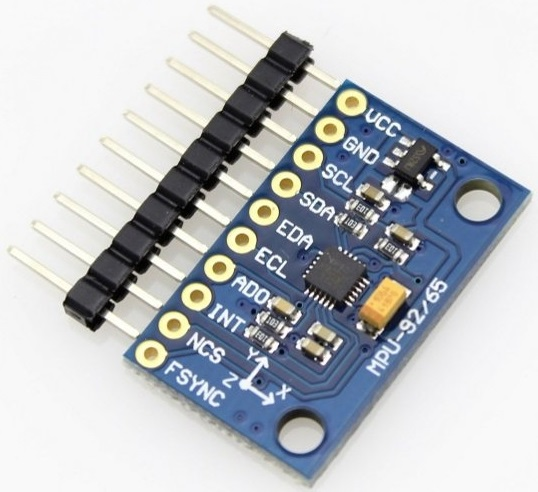
\includegraphics[width=.5\linewidth]{image/imu}
		\end{minipage}%
		\begin{minipage}{.3\textwidth}
			\caption{LIDAR}
			\centering
			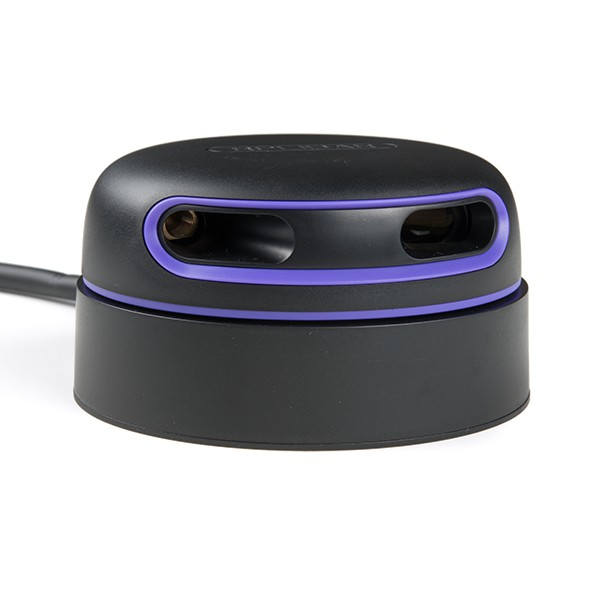
\includegraphics[width=.5\linewidth]{image/lidar}
		\end{minipage}%
		\begin{minipage}{.3\textwidth}
			\begin{block}{LIDAR and IMU Measurement}
				\begin{equation}
					y_k=
					\begin{bmatrix}
						p_{x,k}\\
						p_{y,k}\\
						\omega T_s	
					\end{bmatrix}
				\end{equation}
			\end{block}
		\end{minipage}
	\end{figure}
\end{frame}

%\begin{frame}
%	\frametitle{Mobile Robot and Sensor Model}
%	\framesubtitle{Mobile Robot Kinematic Model}
%	Using Euler approximation, in discrete time step, we get:
%	\begin{block}{Robot pose in discrete time step}
%	\begin{equation}
%		x_k=
%		\begin{bmatrix}
%			p_{x,k}\\
%			p_{x,k}\\
%			\theta_k
%		\end{bmatrix}=
%		\begin{bmatrix}
%			p_{x,k-1} + V_{k-1} T_s cos(\theta_{k-1}) \\
%			p_{y,k-1} + V_{k-1} T_s sin(\theta_{k-1}) \\
%			\theta_{k-1} + \omega_{k-1} T_s\\
%		\end{bmatrix}
%	\end{equation}
%	\end{block}
%	Where:
%	\begin{itemize}
%		\item {\makebox[1cm]{\(V\)\hfill} is the linear velocity in x-axis}
%		\item {\makebox[1cm]{\(\omega\)\hfill} is the angular velocity about z-axis}
%		\item {\makebox[1cm]{\(k\)\hfill} is time step}
%		\item {\makebox[1cm]{\(T_s\)\hfill} is sampling time}
%	\end{itemize}
%	\end{frame}


\begin{frame}
	\frametitle{Mobile Robot and Sensor Model}
	\framesubtitle{Sensor Model}
	In this project, we use sensors for \textbf{Robot Localization} and building \textbf{Occupancy Grid Map}.
	\begin{itemize}
		\item<1-> \textbf{Robot Localization} is a task of determine location of robot inside the map
		\item<2-> \textbf{Occupancy Grid Map} is graph that represents the environment.
	\end{itemize}
	\begin{figure}
		\caption{Localization\footnotemark}
		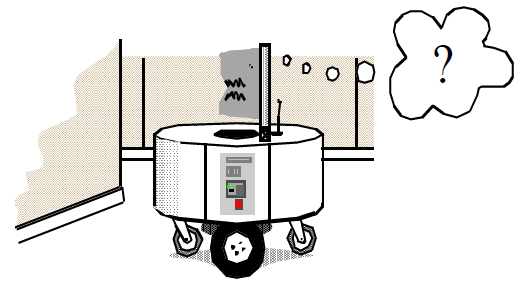
\includegraphics[scale=0.3]{image/robot_wai.png}
	\end{figure}
\footnotetext[5]{https://docplayer.net/26402340-An-introduction-to-mobile-robotics.html}
\end{frame}




\begin{frame}
	\frametitle{Mobile Robot and Sensor Model}
	\begin{block}{Robot Localization}
		We use \textbf{Extended Kalman Filter(EKF)} as sensor fusion for robot localization.
	\end{block}
	\begin{block}{Occupancy Grid Map}
		We use \textbf{Hector SLAM} ROS package to create map.
	\end{block}
\end{frame}


\begin{frame}
	\frametitle{Mobile Robot and Sensor Model}
	\framesubtitle{Sensor Fusion}
	\textbf{Extended Kalman Filter(EKF)} is a state estimation algorithm that estimates the unknown or uncertain variable given the observation. In our case, the states of the system is \(x\)(robot pose)
	\begin{block}{Model Equation}
	\begin{equation}
		x_k = f(x_{k-1},u_{k-1}) + w_{k-1}
	\end{equation}
	\begin{equation}
		y_k = h(x_k) + v_k
	\end{equation}
	\end{block}
	Where:
	\begin{itemize}
		\item {\makebox[1cm]{\(y\)\hfill} is the measurement vector}
		\item {\makebox[1cm]{\(u\)\hfill} is the control input vector}
		\item {\makebox[1cm]{\(w\)\&\(v\)\hfill} are the guassian white noise with covariance \(Q\) and \(R\)} respectively
	\end{itemize}
\end{frame}


\begin{frame}
	\frametitle{Mobile Robot and Sensor Model}
	\framesubtitle{Sensor Fusion}
	\begin{minipage}{.8\textwidth}
	EKF is divided into 2 steps.
	% Table ====================================================================================
	\begin{table}[h]
		\begin{flushleft}
			\caption{Extended Kalman Filter Algorithm}
			\begin{tabular}{lll}
				\hline
				\textbf{Prediction}         && \\
				\hline
				Predicted State estimate    && \(\boxed{\hat{x}^-_k} = f(\hat{x}^-_{k-1},u_{k-1})\) \\
				Predicted error co-variance && \(P^-_k = F_{k-1}P^+_{k-1}F^T_{k-1} + Q\)\\
				\hline
				\textbf{Correction}         && \\
				\hline
				Expected Output             && \(\hat{y}_k = h(\hat{x}^-_k)\)\\
				Measurement residual        && \(\tilde{y}_k = \boxed{y_k} - \hat{y}_k\)\\
				Kalman Gain                 && \(K_k = P^-_kH^T_k(R+H_kP^-_kH^T_k)^{-1}\)\\
				Updated state estimate      && \(\hat{x}^+_k = \hat{x}^-_k + K_k\tilde{y}\)\\
				Updated error co-variance   && \(P^+_k = (I-K_kH_k)P^-_k\)\\
				\hline
			\end{tabular}
		\end{flushleft}
	\end{table}
	\end{minipage}%
	\begin{minipage}{.2\textwidth}
		\begin{flushleft}
		\begin{itemize}
			\item \(F_{k-1}\)
		\end{itemize}
			\[F_{k-1} = \frac{\partial f}{\partial x}|_{\hat{x}^+_{k-1},u_{k-1}}\]
		\begin{itemize}
			\item \(H_k\)
		\end{itemize}
			\[H_k = \frac{\partial h}{\partial x}|_{\hat{x}^-_k}\]
		\end{flushleft}
	\end{minipage}
\end{frame}


\begin{frame}
	\frametitle{Mobile Robot and Sensor Model}
	\framesubtitle{Sensor Fusion}
	Where:
	\begin{itemize}
		\item {\makebox[1cm]{\(Q\)\hfill} is the covariance matrix of prediction model}
		\item {\makebox[1cm]{\(R\)\hfill} is the covariance matrix of measurement model}
		\item {\makebox[1cm]{\(F_{k-1}\)\hfill} is the Jacobian matrix of the nonlinear state function}
		%\[F_{k-1} = \frac{\partial f}{\partial x}|_{\hat{x}^+_{k-1},u_{k-1}}\]
		\item {\makebox[1cm]{\(H_k\)\hfill} is the Jacobian matrix of the nonlinear measurement function}
		%\[H_k = \frac{\partial h}{\partial x}|_{\hat{x}^-_k}\]
	\end{itemize}
\end{frame}



\begin{frame}
	\frametitle{Mobile Robot and Sensor Model}
	\framesubtitle{Architecture}
	\begin{figure}
		%\caption{Architecture}
		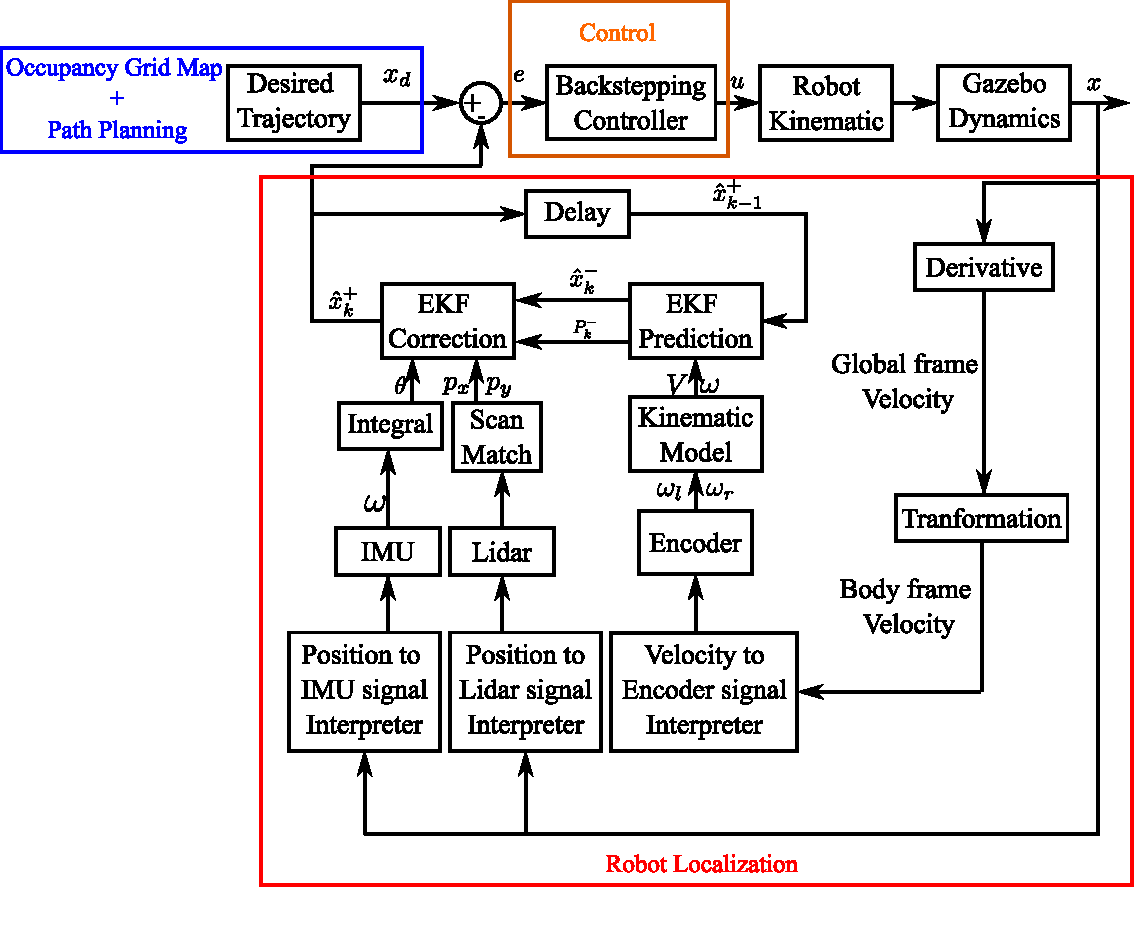
\includegraphics[scale=0.45]{image/arch.pdf}
	\end{figure}
\end{frame}



\begin{frame}
	\frametitle{Mobile Robot and Sensor Model}
	\framesubtitle{Mobile Robot and Sensor in Gazebo Model}
	\begin{figure}
		\caption{Mobile Robot Model in Gazebo}
		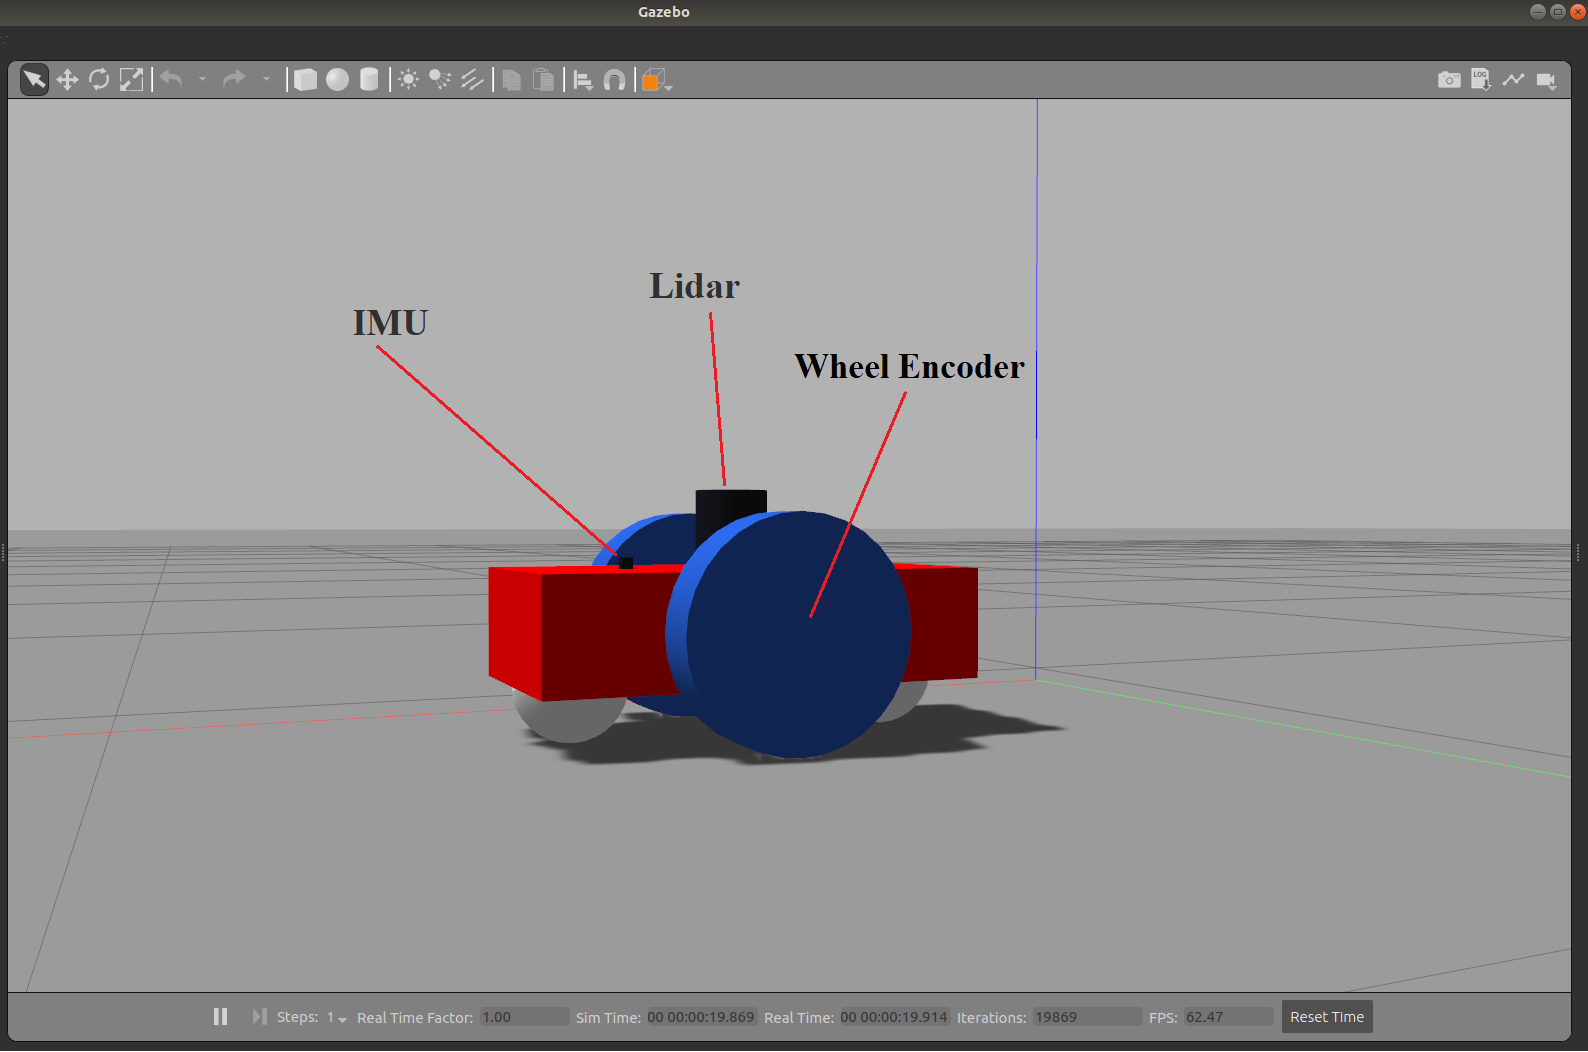
\includegraphics[scale=0.2]{image/Gazebo_sim.png}
	\end{figure}
\end{frame}



\begin{frame}
	\subsection{Occupancy Grid Map}
	\setbeamercolor{block title example}{use=structure,fg=white,bg=blue!80!black}
	\begin{beamercolorbox}[rounded=true]{block title example}
		\centering
		\LARGE
		Occupancy Grid Map
	\end{beamercolorbox}
\end{frame}



\begin{frame}
	\frametitle{Occupancy Grid Map}
	The Occupancy Grid Map is composed of multiple cell together to represents \textbf{Free Space} and \textbf{Obstacle Space} of the surrounding environment.
	\begin{figure}[h]
		\caption{Occupancy Grid Map Example (view in Rviz)}
		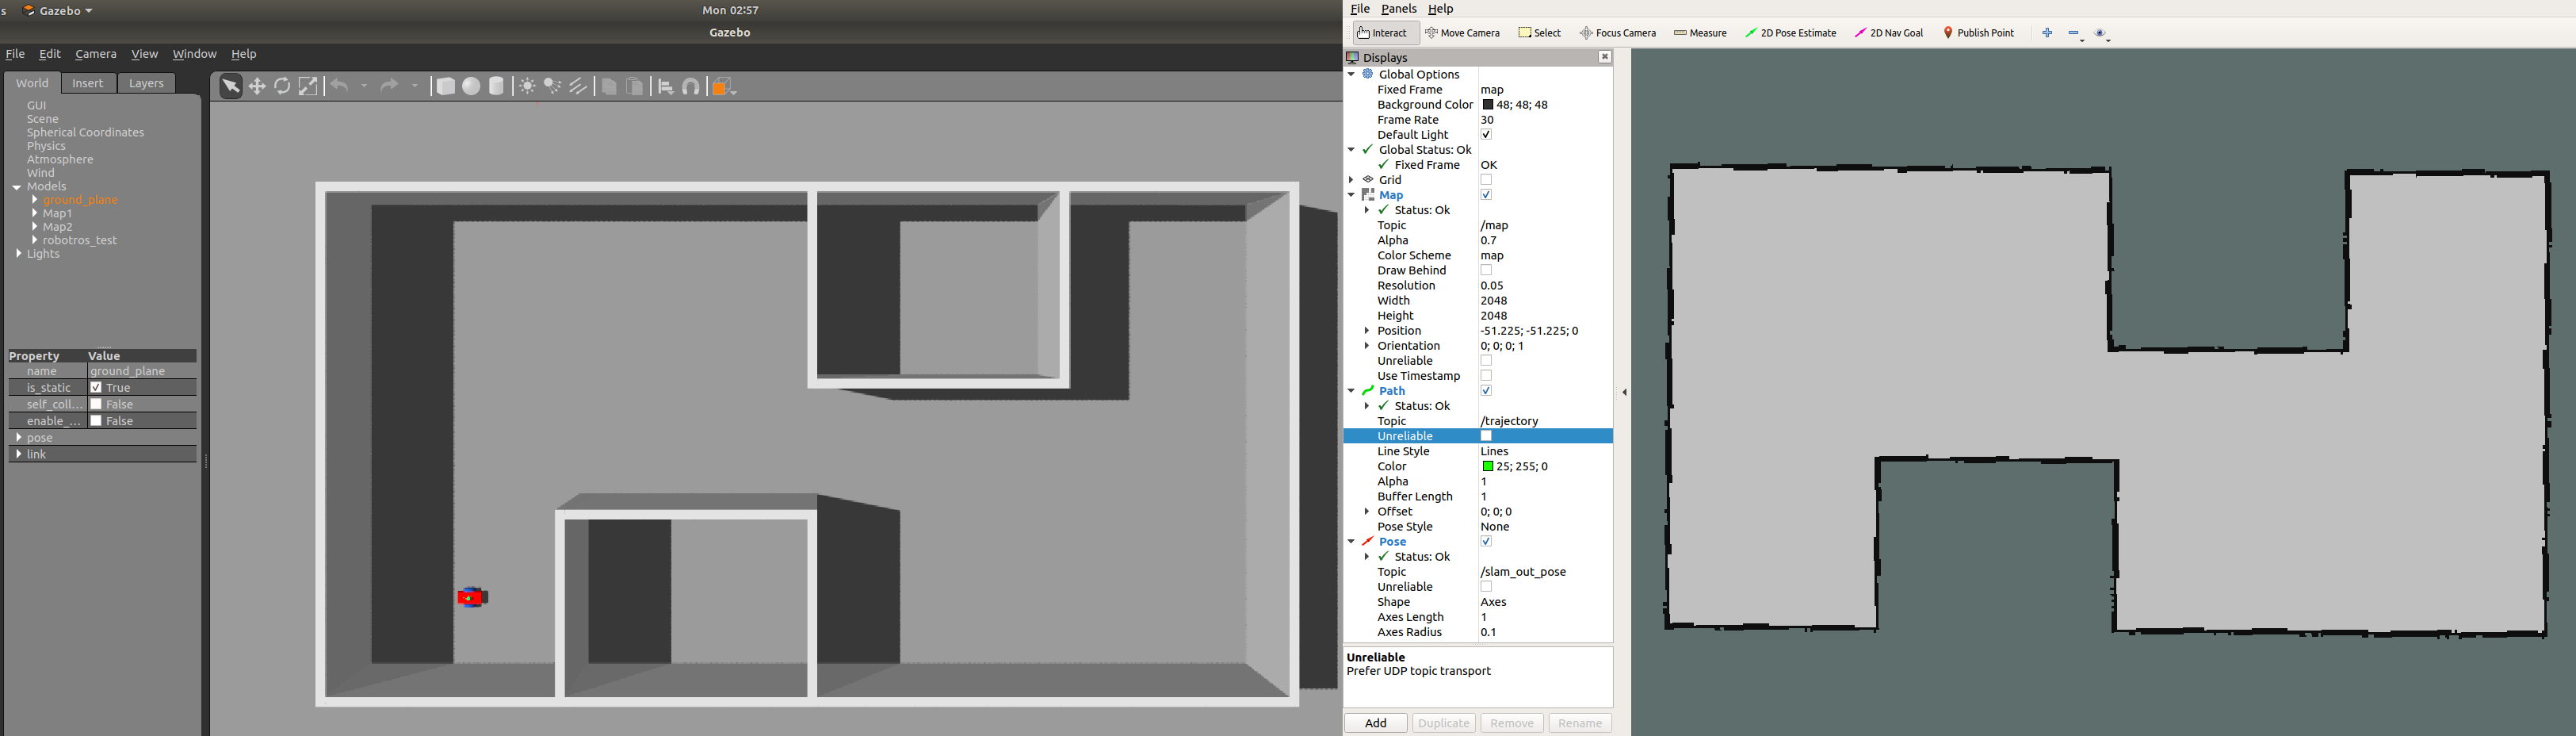
\includegraphics[scale=0.17]{image/map_ex_rviz.png}
	\end{figure}
\end{frame}


\begin{frame}
	\frametitle{Occupancy Grid Map}
	Each cell has its correspond address and a probability value of either 1 or 0 which represents occupied or free respectively.
	\begin{figure}[h]
		\caption{Occupancy Grid Map Cell}
		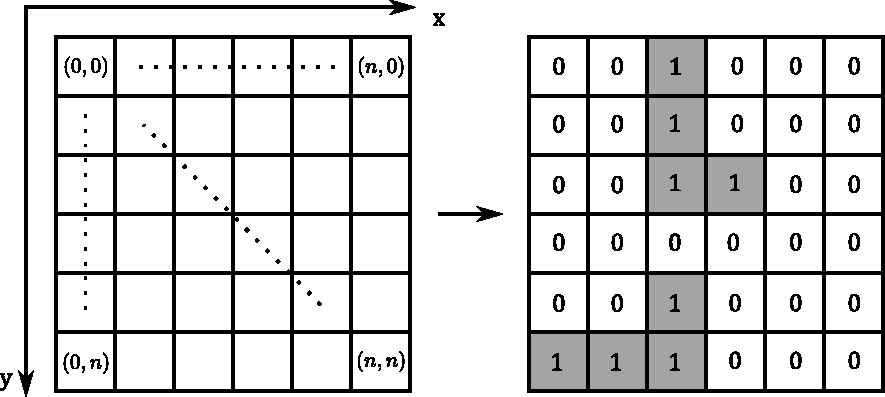
\includegraphics[scale=0.7]{image/ocm_value.pdf}
	\end{figure}
\end{frame}


\begin{frame}
	\frametitle{Occupancy Grid Map}
	\framesubtitle{Simultaneous Localization and Mapping (SLAM)}
	%SLAM use the LIDAR data and the estimated robot pose (Odometry) to construct the Occupancy Grid Map. In this project, we use Hector SLAM ROS package.
	SLAM use Robot and Sensor data that observe from environment to construct the Occupancy Grid Map. In this project, we use Hector SLAM ROS package.
	\begin{columns}
		\column{0.5\textwidth}
		\begin{figure}[h]
			\caption{SLAM work flow}
			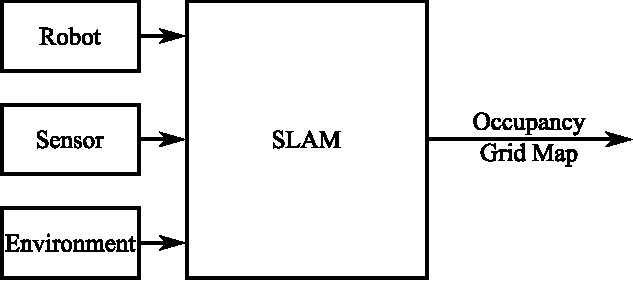
\includegraphics[scale=0.7]{image/slaming.pdf}
		\end{figure}
	
		\column{0.5\textwidth}
		\begin{figure}[h]
			\caption{Hector SLAM\footnotemark}
			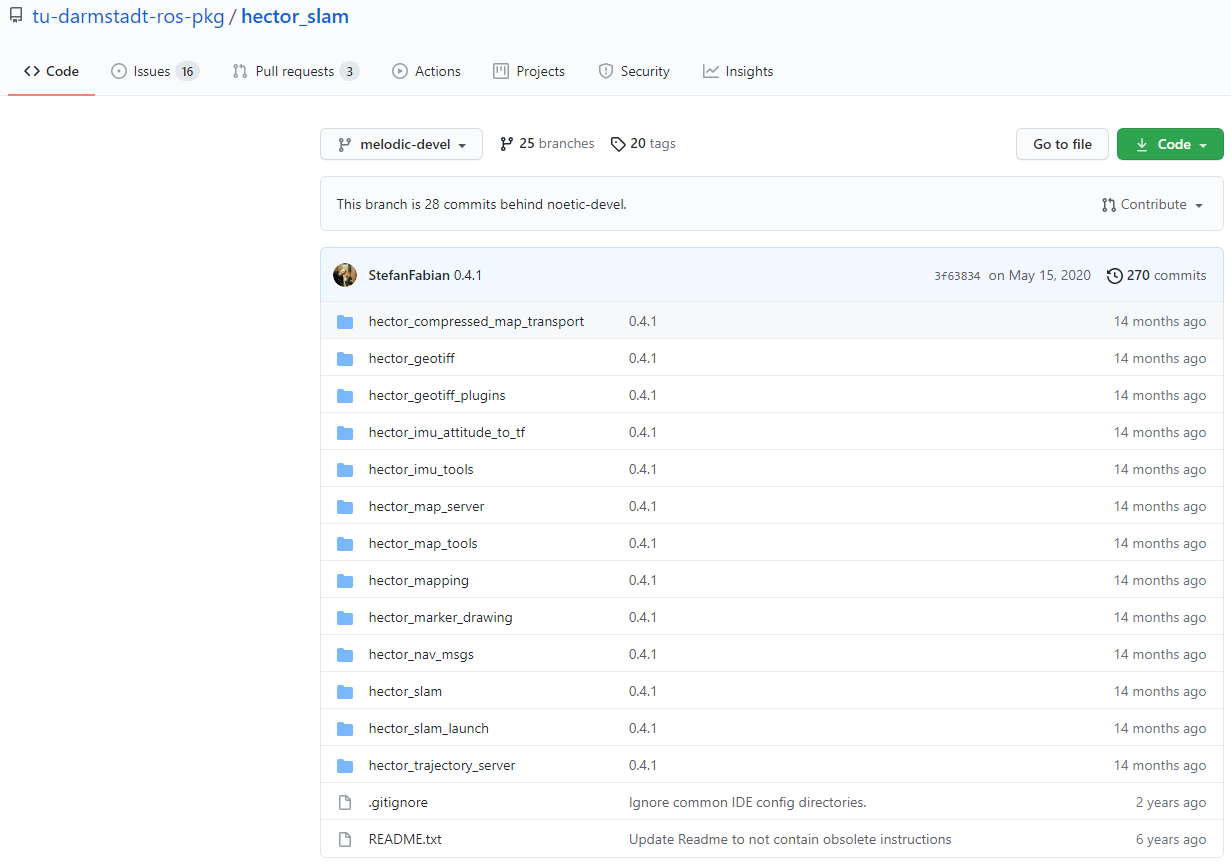
\includegraphics[scale=0.15]{image/hector.png}
		\end{figure}
	\end{columns}
\footnotetext[6]{https://github.com/tu-darmstadt-ros-pkg/hector\_slam}
\end{frame}



\begin{frame}
	\subsection{Path Planning}
	\setbeamercolor{block title example}{use=structure,fg=white,bg=blue!80!black}
	\begin{beamercolorbox}[rounded=true]{block title example}
		\centering
		\LARGE
		Path Planning
	\end{beamercolorbox}
\end{frame}



\begin{frame}
	\frametitle{Path Planning}
	\begin{itemize}
		\item<1-> Path Planning is a process of finding the pathway to move from point A to point B.
		\item<2-> In mobile robot navigation, Path Planning is commonly used for finding the pathway to move the robot inside the surrounding environment.
	\end{itemize}
\end{frame}



\begin{frame}
	\frametitle{Path Planning}
	\framesubtitle{A* Algorithm}
	A* algorithm is an algorithm that based on the heuristic method. A* is the optimal best-first search algorithm.
	\begin{block}{Cost function}
		\begin{equation}
			F(n)=G(n)+H(n)
		\end{equation}
	\end{block}
	Where:
	\begin{itemize}
		\item {\makebox[1cm]{\(F\)\hfill} is the total cost of node path}
		\item {\makebox[1cm]{\(G\)\hfill} is the exact distance from the starting node to the current node}
		\item {\makebox[1cm]{\(H\)\hfill} is the estimation distance from the current node to the ending node}
		\item {\makebox[1cm]{\(n\)\hfill} is the node}
	\end{itemize}
\end{frame}



\begin{frame}
	\frametitle{Path Planning}
	\framesubtitle{A* Algorithm}
	G and H value is calculated using Euclidean distance formula.
	\begin{block}{Euclidean Distance}
		\begin{equation}
			d_{ab} = \sqrt{(x_b - x_a)^2 + (y_b - y_a)^2}
		\end{equation}
	\end{block}
	\begin{figure}
		\caption{Occupancy Grid Cell in A*}
		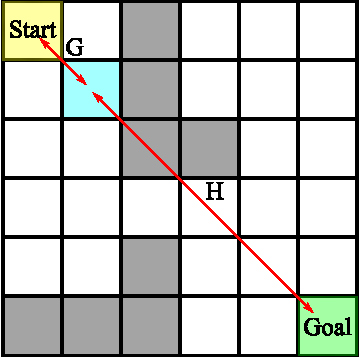
\includegraphics[scale=0.6]{image/astar_eudis.pdf}
	\end{figure}
\end{frame}



\begin{frame}
	\frametitle{Path Planning}
	\framesubtitle{A* Algorithm}
	\begin{itemize}
		\item A* search for pathway from \textbf{Start} node to the \textbf{Goal} node by expanding node.
		\item Node Expansion is to calculate the travel cost from the current node to the neighbor node. The lowest travel cost node is chosen.
	\end{itemize}
	
	
	\begin{figure}
		\caption{A* path finding from Start to Goal}
		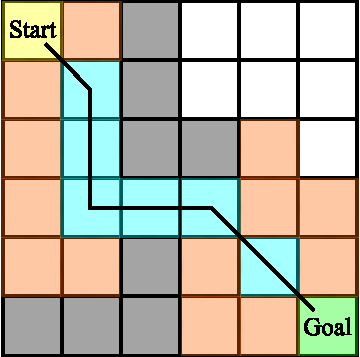
\includegraphics[scale=0.6]{image/astar_stog.pdf}
	\end{figure}
\end{frame}



\begin{frame}
	\subsection{Control}
	\setbeamercolor{block title example}{use=structure,fg=white,bg=blue!80!black}
	\begin{beamercolorbox}[rounded=true]{block title example}
		\centering
		\LARGE
		Control
	\end{beamercolorbox}
\end{frame}



\begin{frame}
	\frametitle{Control}
	In Mobile Robot Navigation, controller is used to control robot motion.\\ \pause
	\hspace{\linewidth}\\
	For the Differential Drive Mobile Robot, we want to control:
	\begin{itemize}
		\item \(V\)
		\item \(\omega\)
	\end{itemize}
	\pause
	\hspace{\linewidth}\\
	Most commonly known control method are:
	\begin{itemize}
		\item Reference point control
		\item Segment of line control
		\item Trajectory control
	\end{itemize}
\end{frame}


\begin{frame}
	\frametitle{Control}
	\framesubtitle{Backstepping Controller}
	Backstepping Controller is one type of the trajectory controller.
	\begin{columns}
		\column{0.5\textwidth}
		\begin{figure}
			\caption{Differential Drive Control}
			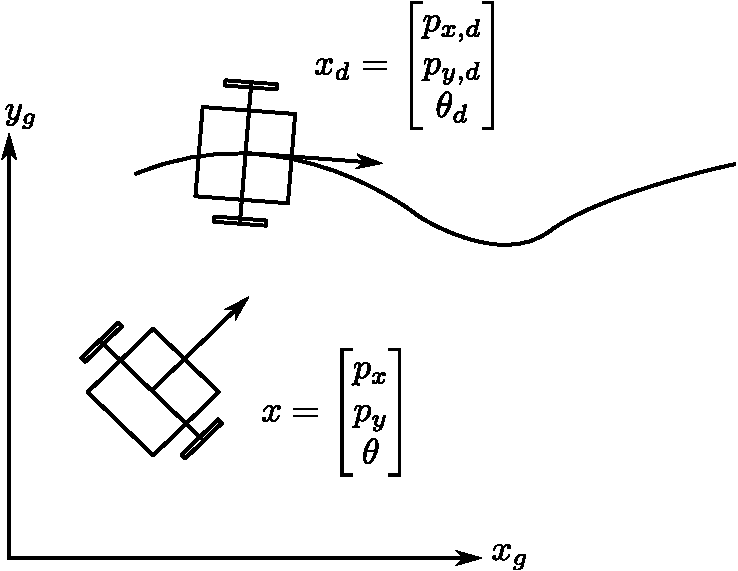
\includegraphics[scale=0.5]{image/cont.pdf}
		\end{figure}
		\column{0.5\textwidth}
		Controller nullify the error between the \(x\) and \(x_d\).
		\begin{block}{Error Model}
			\begin{equation}
				\begin{bmatrix}
					e_1\\
					e_2\\
					e_3
				\end{bmatrix}=\begin{bmatrix}
				cos\theta && sin\theta && 0\\
				-sin\theta && cos\theta && 0\\
				0 && 0 && 1
			\end{bmatrix}
			\begin{bmatrix}
				p_{x,d} - p_x\\
				p_{y,d} - p_y\\
				\theta_d - \theta
			\end{bmatrix}
			\end{equation}
		\end{block}
	\end{columns}
\end{frame}


\begin{frame}
	\frametitle{Control}
	\framesubtitle{Backstepping Controller}
	Proving by the Lyapunov stability\footnotemark, the controllers produce the control input for the robot are:
	\begin{columns}
		\column{0.5\textwidth}
		\begin{block}{Control}
			\begin{equation}
				\begin{bmatrix}
					V_c\\
					\omega_c
				\end{bmatrix} = 
				\begin{bmatrix}
					V_{ref} cos e_3 + k_1e_1\\
					\omega_{ref} + k_2 V_{ref} e_2 + k_2 sin e_3
				\end{bmatrix}
			\end{equation}
		\end{block}
		\column{0.5\textwidth}
		Where:
		\begin{itemize}
			\item {\makebox[1.5cm]{\(k_1,k_2,k_3\)\hfill} are positive constants for tuning}
			\item {\makebox[1.5cm]{\(V_c\)\hfill} is linear velocity control}
			\item {\makebox[1.5cm]{\(\omega_c\)\hfill} is angular velocity control}
			\item {\makebox[1.5cm]{\(V_{ref}\)\hfill} is reference linear velocity}
			\item {\makebox[1.5cm]{\(\omega_{ref}\)\hfill} is reference angular velocity}
		\end{itemize}
	\end{columns}
\footnotetext[7]{G. Zidani et al., "Backstepping controller for a wheeled mobile robot," 2015 4th International Conference on Systems and Control (ICSC)}
\end{frame}



\begin{frame}
	\frametitle{Control}
	\framesubtitle{Architecture}
	\begin{figure}
		%\caption{Architecture}
		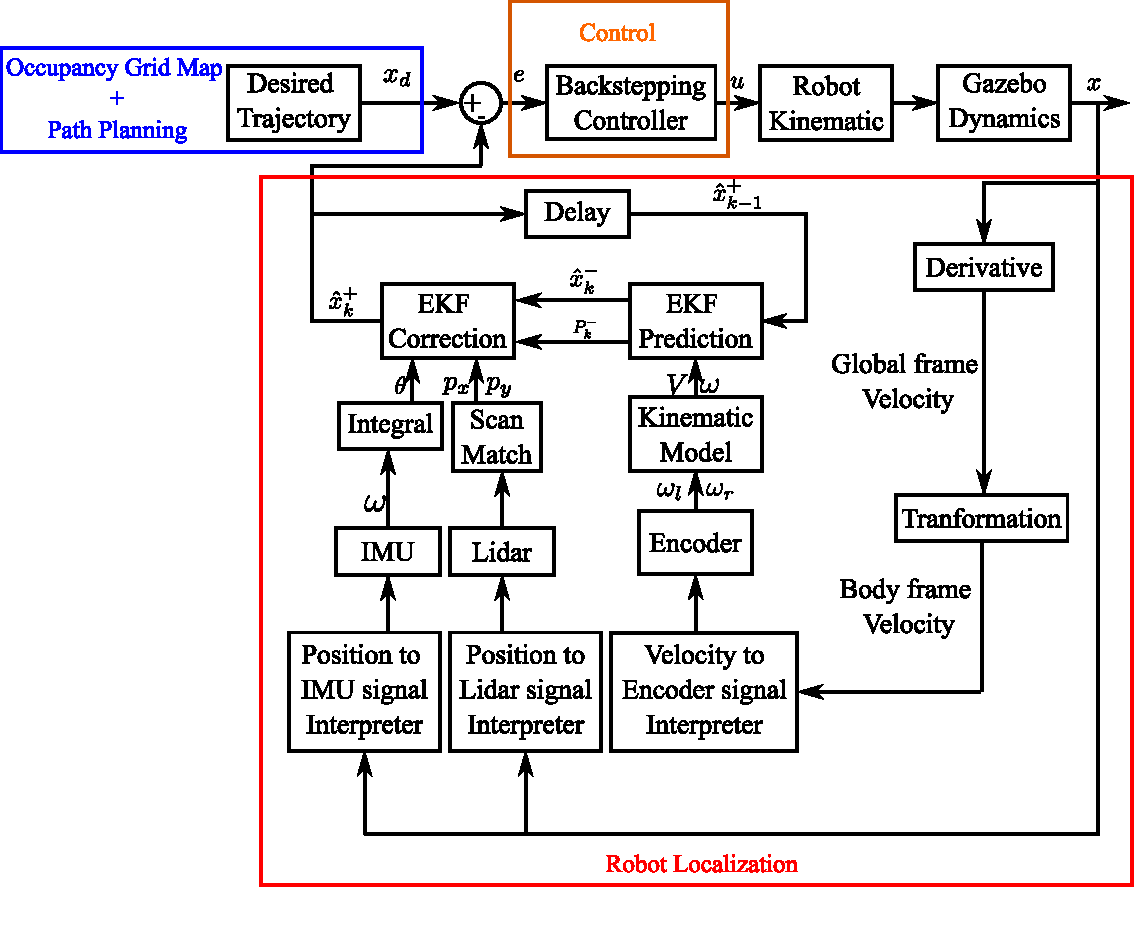
\includegraphics[scale=0.45]{image/arch.pdf}
	\end{figure}
\end{frame}